Our goal now is to show that, in view of its compactness, our minimal blow-up solution cannot exist, completing the proof of Theorem \ref{thm:ESS}. We cite \cite{KenigKoch2011}. The strategy can be summarised by the following figure:


\begin{figure}[h]
	\begin{center}
		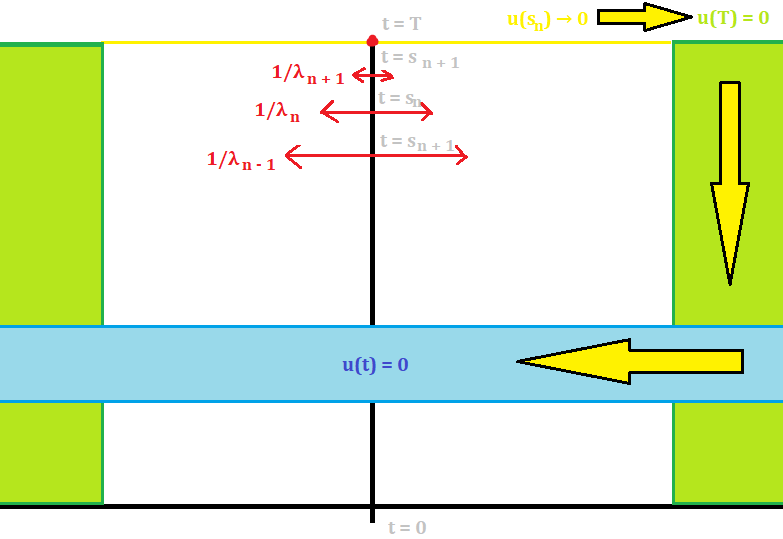
\includegraphics[scale = 0.7]{graphics/rigidity}
		\caption{By compactness, minimal blow-up solutions cannot have any radiation, i.e. $u_{\mathrm{crit}}(t) \rightharpoonup 0$ as $t \to T^*$, since it concentrates into small scales $1/\lambda_n \to 0$. We know $u_{\mathrm{crit}} \in L^\infty_t L^3_x [0, T^*)$, so we can find a large ball outside of which $u_{\mathrm{crit}}$ is small in $L^3_{t, x}$-norm, and therefore smooth by partial regularity. Backwards uniqueness implies $u_{\mathrm{crit}} \equiv 0$ outside this ball for all time, while unique continuation extends this to an entire time-slice.  }
	\end{center}\label{fig:1}
\end{figure}

We first show that the minimal blow-up solution does not have ``radiation'', that is, $u_{\mathrm{crit}} \to 0$ weakly approaching the blow-up time $t \uparrow T^*$. Indeed, this should hold in view of compactness, which states that the entirety of the $L^3$-norm of $u_{\mathrm{crit}}$ concentrates into smaller scales. 

\begin{proposition}[No radiation]
	Let $u_{\mathrm{crit}}$ be a minimal blow-up solution, then $u_{\mathrm{crit}} \to 0$ in $L^2_{\loc} (\R^3)$ along some sequence of times approaching the blow-up time. 
\end{proposition}

\begin{proof}
	Recall that there exists a sequence
	\[
		v_n (x) := \frac{1}{\lambda_n} u\left(s_n, \frac{x - x_n}{\lambda_n}\right)
	\]
with $s_n \uparrow T^*$ and $\lambda_n \to + \infty$ which converges in $L^3$ to some $v$. Almost periodic solutions satisfy $u(s_n) \to 0$ in the sense of distributions. Indeed, we compute
	\begin{align*}
		\int_{|x| \leq R} |u(s_n, x)|^2 \, dx 
			&= \int_{|x| \leq R} |\lambda_n v_n (\lambda_n x + x_n)|^2 \, dx \\
			&= (\lambda_n)^{-1} \int_{|y - x_n| \leq \lambda_n R} |v_n(y)|^2 \, dy\\
			&=  (\lambda_n)^{-1} \left(\int_{\substack{|y - x_n| \leq \lambda_n R \\ |y| \leq \epsilon \lambda_n R}} + \int_{\substack{|y - x_n| \leq \lambda_n R \\ |y| > \epsilon \lambda_n R}}\right) |v_n(y)|^2 \, dy . 
	\end{align*}	
Then by Holder
	\begin{align*}
		\frac{1}{\lambda_n}\int_{\substack{|y - x_n| \leq \lambda_n R \\ |y| \leq \epsilon \lambda_n R}}  |v_n(y)|^2 \, dy
			&\leq \frac{1}{\lambda_n} ||v_n||_{L^3}^2 |\{ |y| \leq \epsilon \lambda_n R \}|^{1/3} \\
			&\lesssim A^2 \epsilon R
	\end{align*}
and
	\begin{align*}
		\frac{1}{\lambda_n}\int_{\substack{|y - x_n| \leq \lambda_n R \\ |y| > \epsilon \lambda_n R}}  |v_n(y)|^2 \, dy
			&\leq  \frac{1}{\lambda_n} ||v_n||_{L^3 (|y| > \epsilon \lambda_n R)}^2 |\{|y - x_n| \leq \lambda_n R \}|^{1/3} \\
			&\lesssim R ||v_n||_{L^3 (|y| > \epsilon \lambda_n R)}^2
	\end{align*}
	Sending $n \to \infty$ implies the second term goes to zero by dominated convergence, then sending $\epsilon \to 0$ shows the first goes to zero. 
\end{proof}



\begin{theorem}[$\epsilon$-regularity criterion, \cite{CaffarelliEtAl1982, Lin1998}]\label{thm:epsilon}
	There exists $\epsilon \ll 1$ such that for any weak solution $u$ to Navier-Stokes \eqref{NS} satisfying the scale-invariant estimate in a parabolic cylinder
		\[
			\frac{1}{r^2} \iint_{Q_r (t_0, x_0)} (|u|^3 + |p|^{3/2}) \, dx dt \leq \epsilon
		\]
	is smooth in space in the smaller parabolic cylinder $Q_{r/2} (t_0, x_0)$.  
\end{theorem}


\begin{proposition}[Unique continuation]\label{prop:unique1}
	Suppose $w$ is a smooth function which 
		\begin{itemize}
			\item has regularity $w, \partial_t w, \nabla w, \nabla^2 w \in L^2_{\loc, t, x}$, 
			
			\item satisfies the vanishing condition near the origin $|w| \lesssim_k (|x| + |t|^{1/2})^k$, 
			
			\item satisfies the differential inequality $|\partial_t w - \Delta w| \lesssim |\nabla w| + |w|$, 
		\end{itemize}
	on the region $(-T, 0) \times B_r$. Then $w(0) \equiv 0$ on the ball $B_r$. 
\end{proposition}

\begin{proposition}[Backwards uniqueness]\label{prop:backunique1}
	Suppose $w$ is a smooth function which
		\begin{itemize}
			\item has regularity $w, \partial_t w, \nabla w, \nabla^2 w \in L^2_{\loc, t, x}$, 
			\item satisfies the growth condition $|w| \leq e^{M |x|^2}$, 
			\item satisfies the differential inequality $|\partial_t w - \Delta w| \lesssim |\nabla w| + |w|$,  
		\end{itemize}
	on the region $(-T, 0) \times (\R^3 \setminus B_R)$. If $w$ vanishes at time $t = 0$ on the region $\R^3 \setminus B_R$, then it vanishes backwards in time on $(-T, 0) \times (\R^3 \setminus B_R)$. 
\end{proposition}

Let us complete the proof of the theorem. Since $u \in L^\infty_t L^3_x ([0, T^*) \times \R^3)$, we also have $u \in L^3_{t, x} ([0, T^*) \times \R^3)$. By dominated convergence theorem, there exists $R \gg 0$ such that 
	\[
		\int_0^{T^*} \int_{|x| \geq R} |u|^3 + |p|^{3/2} \, dx dt \ll \epsilon.
	\]
It follows from the $\epsilon$-regularity theorem that $u$ is smooth in space in the exterior region $|x| \gg R$. We pass to the vorticity, which satisfies the equation 
	\[
		\partial_t \omega - \Delta \omega = (\omega \cdot \nabla) u - (u \cdot \nabla \omega). 
	\]
Since $u$ and therefore $\omega$ vanishes in the exterior region, the conditions for backwards uniqueness are trivially satisfied, so we know that the vorticity vanishes in this exterior region for all time. On the other hand, regularity theorem strictly between the blow-up time and the initial time, e.g. $(\epsilon, T^* - \epsilon)$, furnishes pointwise bounds for $u$ and $\nabla u$, allowing us to apply unique continuation to conclude $\omega \equiv 0$ and thus also $u \equiv 0$. 

\begin{remark}
	It is interesting to think about whether this method could be adapted to give alternative proofs of rigidity for other critical problems. Indeed, as remarked in Escauriaza-Seregin-Sverak,
	
\begin{quote}
	one could speculate that the general idea of [backwards uniqueness] is applicable to an even larger class of interesting equations with critical non-linearities, such as non-linear Schrodinger equations or non-linear wave equations. However, local regularity seems to be a more complicated problem in these cases than in the parabolic case. \hfill ---\cite{EscauriazaEtAl2003}
\end{quote}

The key obstruction seems to be the lack of any partial regularity theory such as Theorem \ref{thm:epsilon} for non-linear dispersive equations. 
\end{remark}
